\documentclass{article}
\usepackage{amsmath,amsthm,amssymb}
\usepackage{mathtext}
\usepackage[T2A]{fontenc}
\usepackage[utf8]{inputenc}
\usepackage[english]{babel}
\usepackage{graphicx}
\usepackage{hyperref}
\usepackage{multirow}
\usepackage[backend=biber]{biblatex}
\addbibresource{bib.bib}

\setlength{\arrayrulewidth}{0.5mm}
\setlength{\tabcolsep}{18pt}


\title{Move-by-Move Commentary for Chess Games}
\author{Gavrilyuk Alexander}
\date{May 2024}



\begin{document}
\maketitle
\begin{abstract}
    This paper gives a brief overview of the problem of generating natural language descriptions of chess games and describes my attempt to contribute in the process of solving it.
    
    Project code is located here: \url{https://github.com/CrubBucket/NLP_chess_commentary}.
\end{abstract}



\section{Introduction}
The problem of automatic chess games descriptions generation is not quite popular among non-chess community, but is crucial for chess enthusiasts. Having a tool to generate high-quality comments for each move in a chess game would make an education process easier and more pleasant for players. Nowadays we have very strong chess engines which can easily beat any grand-master but studying lines these engines provide can be quite complicated because of the lack of explanations. So, NLP-approach can fix it and add more humanity to raw machine analysis.
\subsection{Team}

\textbf{Gavrilyuk Alexander}



\section{Related Work}
\label{sec:related}
There are not so many papers and works related to this topic due to its unpopularity. One of the most detailed and resent ones is a paper \href{https://aclanthology.org/P18-1154/}{"Learning to Generate Move-by-Move Commentary for Chess Games from Large-Scale Social Forum Data"}\cite{article}

First of all, authors introduce a new large-scale chess commentary dataset consists of 298K aligned game move/commentary pairs (table 1)~\ref{table:1}~\ref{table:2}. The dataset \textit{D} consists of data points of the form $(Si, Mi, Gi), i \in \{1, 2, .., |D|\}$ where $S_i$ is the commentary text for move $M_i$ and $G_i$ is the corresponding chess game. $S_{i_1}$ is a sequence of m tokens $S_{i_1}, S_{i_2}, ..., S_{i_m}$, so the solution of the move commentary boils down to modeling the probability $P(S_i|M_i, C_i, R_i)$, where $C_i$ and $Ri$ are current and previous board stages.

Authors consider the following features to provide their model with necessary information to generate commentary texts:

\begin{itemize}
\item \textbf{Move} features $f_{move}(M_i, C_i, R_i)$ - encode the general current move information
\item \textbf{Threat} features $f_{threat}(M_i, C_i, R_i)$ - encode information about pieces of opposite player attacking the moved piece before and after the move
\item \textbf{Score} features $f_{score}(M_i, C_i, R_i)$ - capture the quality of move and general progress of the game
\end{itemize}

Representing of all these features is considered through embeddings. For categorical features we authors directly look up the embedding using corresponding token, while real valued features are encoded by first binning them and then using corresponding number for embedding lookup. Let $E$ represent the embedding matrix. Then $E[f^j_{move}]$ represents embeddings of $j_th$ move feature, or in general $E[f_{move}]$ represents the concatenated embeddings of all move features. Similarly, $E(f_{move}, f_{threat}, f_{score})$ represents concatenated embeddings of all the features.
Finally, authors' model contain LSTM as a decoder. At every output step, the LSTM decoder predicts a distribution over vocabulary words to construct a commentary output. Figure 1~\ref{fig:1} demonstrates a schematic model overview.

\begin{figure}
    \centering
    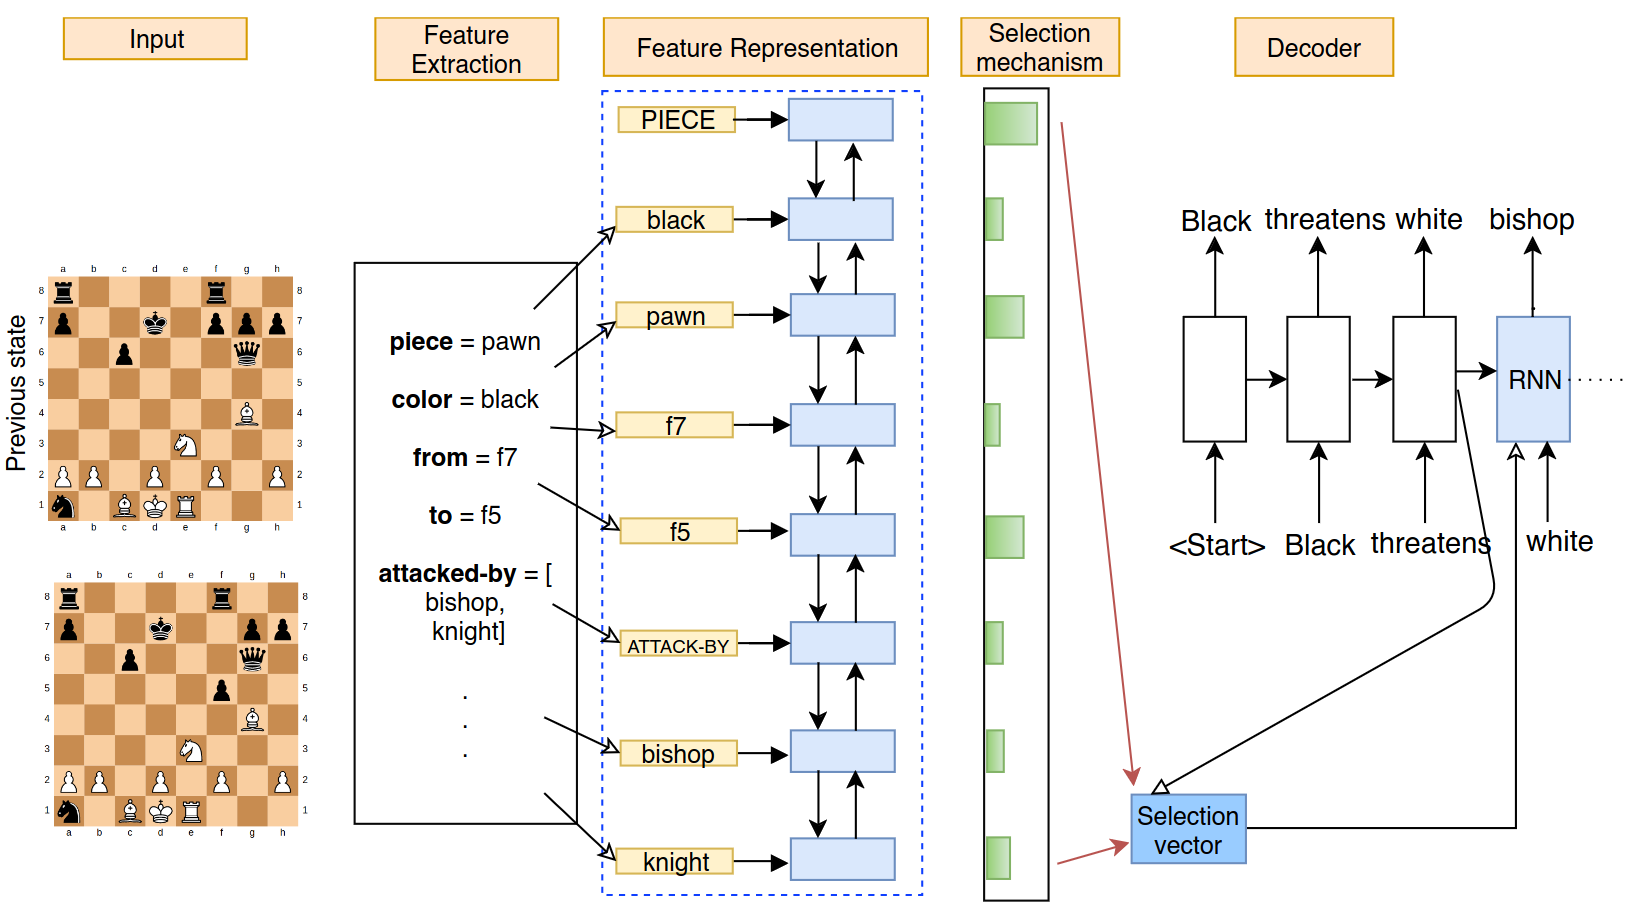
\includegraphics[width = 12cm]{fig_1.png}
    \caption{A model overview.}
    \label{fig:1}
    \end{figure}

Authors mainly observe BLEU and BLEU-2 scores to measure the performance of the models and conduct a human evaluation study.~\ref{table:3}~\ref{table:4}

\begin{table}
\centering
\begin{tabular}{ |p{3cm}|p{3cm}|p{3cm}|  }
\hline
\multicolumn{2}{|c|}{Dataset stats} \\
\hline
Total Games & 11,578 \\
Total Moves & 298,008 \\
Average no. of recorded steps in a game & 25.73 \\
\hline
Frequent Word Types    & 39,424 \\
Rare Word Types & 167,321 \\
\hline
Average Comment Length & 20.55   \\
Long Comments  & 230745 (77\%)\\
\hline
\end{tabular}
\caption{Dataset and Vocabulary Statistics}
\label{table:1}
\end{table}

\begin{table}
\centering
\begin{tabular}{|p{3cm}|p{3cm}|p{1cm}|p{1cm}|}
\hline
\textbf{Category} & \textbf{Example} & \textbf{\% in data} & \textbf{Val acc.} \\
\hline
% \multicolumn{3}{|c|}{Dataset stats} \\
Direct Move Description & An attack on the queen & 31.4\% & 71\% \\
\hline
Move Quality & A rook blunder. & 8.0\% & 90\% \\
\hline
Comparative & At this stage I figured I better move my knight. & 3.7\% & 77.7\% \\
\hline
Planning / Rationale & Trying to force a way to eliminate d5 and prevent Bb5. & 31.2\% & 65\% \\
\hline
Contextual Game Info & Somehow, the game I should have lost turned around in my favor. & 12.6\% & 87\% \\
\hline
General Comment & Protect Calvin , Hobbs & 29.9\% & 78\% \\
\hline
\end{tabular}
\caption{Commentary classification}
\label{table:2}
\end{table}

\begin{table}
\centering
\begin{tabular}{|p{3cm}|p{1cm}|p{1cm}|}
\hline
\textbf{Features} & \textbf{BLEU} & \textbf{BLEU-2} \\
\hline
M & 1.69 & 20.66 \\
M+T & 1.94 & 24.11 \\
M+T+S & 2.02 & 24.70 \\ 
\hline
\end{tabular}
\caption{Results of main model learned on the whole training set using different combinations of features (M - move features, T - threat features, S - score features)}
\label{table:3}
\end{table}

\begin{table}
\centering
\begin{tabular}{|p{3cm}|p{1cm}|p{1cm}|p{1cm}|p{1.5cm}|}
\hline
\textbf{Question} & \textbf{GT} & \textbf{GAC
(M)} & \textbf{GAC
(M+T)} & \textbf{GAC
(M+T+S)} \\
\hline
Is commentary correct for the given move? (\%Yes) & 70.4 & 42.3 & 64.8 & 67.6 \\ 
\hline
Can the move be inferred from the commentary? (\%Yes) & 45.1 & 25.3 & 42.3 & 36.7 \\
\hline
Fluency (scale of (least)1 - 5(most) ) Mean (Std. dev.) & 4.03 (1.31) & 4.15 (1.20) & 4.44 (1.02) & 4.54 (0.89) \\
\hline
\end{tabular}
\caption{Human study results (GT - ground truth, GAC - main model)}
\label{table:4}
\end{table}


\section{Model Description}

Unfortunately, I did not manage to finish this project during the course, but here are some thoughts on how I would modify the architecture given above: 

\begin{itemize}
\item Using GRU instead of LSTM (at least, if they perform similarly, we could reduce the computational expenses).
\item Extending the feature types extracted from different board stages.
\item Considering more chess board stages (not only current and previous ones).
\item Changing strateges for calculating embeddings.
\item Experimenting with ensembling separately trained models.
\end{itemize}


\section{Dataset}
As it was mentioned above, there is a lack of works related to this topic due to its unpopularity, so the main dataset used in this project is the one from \href{https://aclanthology.org/P18-1154/}{previously described paper}. It can be collected with the \href{https://github.com/harsh19/ChessCommentaryGeneration/tree/master}{open-source code}\cite{jhamtani2018acl} provided by authors (as it is totally available for the research purposes).

It is decided to enrich the given dataset with some additional data, which was mined through parsing open \href{https://database.lichess.org/}{Lichess database}. 5.7k moves of 56 games of Candidates Tournament 2024 followed by professional commentary were parsed. Presumably, top level chess content could improve the dataset quality and give some boost to model results. For example, a new category "Professional commentary" can be added to the list of comments classes.

On the Tab.~\ref{table:statistics} you can see the statistics for the mentioned dataset.

\begin{table}
\centering
\begin{tabular}{|p{3cm}|p{1cm}|}
\hline
\multicolumn{2}{|c|}{Dataset stats} \\
\hline
Total Games & 56 \\
Total Moves & 5665 \\
\hline
New words & 3207 \\
\hline
Average Comment Length & 23.06   \\
\hline
\end{tabular}
\caption{Additional Dataset and Vocabulary Statistics}
\label{table:statistics}
\end{table}

Additional dataset contain move notation, FEN notation (to extract all the features connected with pieces placement), current engine evaluation of the position after the certain move and a comment itself. 

\section{Conclusion}
This work is my starting point of a big NLP-project dedicated to automatic chess games commentary generation. Unfortunately, only related works have been studied and a strategy to collect new data and extend existing dataset have been formulated, but the project will undergo further development. If you are interested in this topic, you can spectate this work's growth or even contribute to it via the repository: \url{https://github.com/yournickname/your-project-name}

% \bibliographystyle{apalike}
% \bibliography{lit}

\printbibliography %Prints bibliography

\end{document}
